\documentclass[tikz,border=5pt]{standalone}
\usepackage[UTF8]{ctex}
\usepackage{amsmath,amssymb}
\usetikzlibrary{arrows.meta,calc,angles,quotes,patterns,decorations.pathmorphing}
\definecolor{field}{HTML}{176B9B}
\definecolor{force}{HTML}{B64B32}
\tikzset{>=Latex,line width=.8pt,every node/.style={font=\small},field/.style={color=field},force/.style={color=force},body/.style={draw=black,fill=blue!6},ghost/.style={dashed,gray},labelbox/.style={fill=white,inner sep=1.5pt}}
\begin{document}
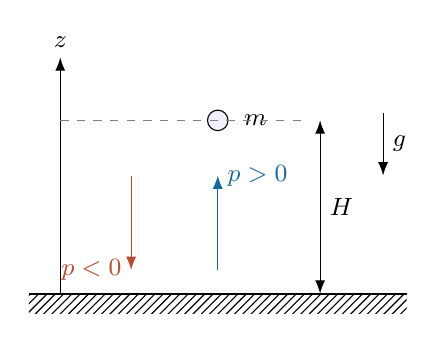
\begin{tikzpicture}
\fill[pattern=north east lines](0,-.25)rectangle(4.8,0);
\draw[thick](0,0)--(4.8,0);
\draw[->](.4,0)--(.4,3)node[above]{$z$};
\draw[body](2.4,2.2)circle(.13)node[right=6pt]{$m$};
\draw[->,field](2.4,.3)--(2.4,1.5)node[right]{$p>0$};
\draw[->,force](1.3,1.5)--(1.3,.3)node[left]{$p<0$};
\draw[ghost](.4,2.2)--(3.5,2.2);
\draw[<->](3.7,0)--(3.7,2.2)node[midway,right]{$H$};
\draw[->](4.5,2.3)--(4.5,1.5)node[midway,right]{$g$};
\end{tikzpicture}
\begin{tikzpicture}
\draw[->](0,0)--(5,0)node[right]{$z$};
\draw[->](0,0)--(0,3.4)node[above]{$V$};
\draw[force,thick](0,0)--(4.7,3.13)node[right]{$mgz$};
\draw[field](0,2.1)--(4.7,2.1)node[right]{$E$};
\draw[ghost](3.15,0)--(3.15,2.1);
\node[below]at(3.15,0){$H$};
\draw[thick](0,0)--(0,3);
\node[left,align=right]at(-.15,1.6){硬壁\\$\psi(0)=0$};
\node[above]at(1.35,2.35){经典允许区};
\node[below]at(4,1.6){禁阻区};
\end{tikzpicture}
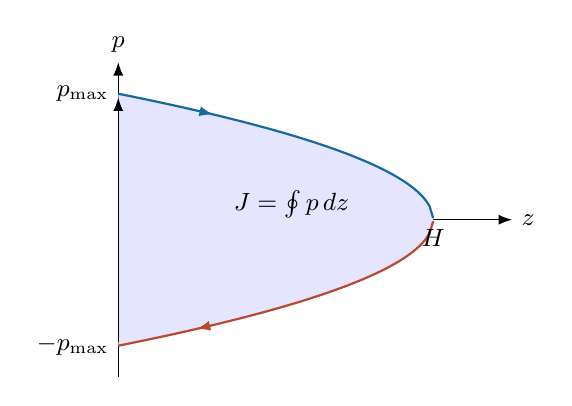
\begin{tikzpicture}
\draw[->](0,0)--(5,0)node[right]{$z$};
\draw[->](0,-2)--(0,2)node[above]{$p$};
\path[fill=blue!10]plot[domain=0:4,samples=90](\x,{1.6*sqrt(max(0,1-\x/4))})
--plot[domain=4:0,samples=90](\x,{-1.6*sqrt(max(0,1-\x/4))})--cycle;
\draw[field,thick,domain=0:4,samples=90]plot(\x,{1.6*sqrt(max(0,1-\x/4))});
\draw[force,thick,domain=0:4,samples=90]plot(\x,{-1.6*sqrt(max(0,1-\x/4))});
\draw[->,field](1,1.3856)--(1.2,1.3387);
\draw[->,force](1.2,-1.3387)--(1,-1.3856);
\draw[->](0,-1.55)--(0,1.55);
\node[left]at(0,1.6){$p_{\max}$};\node[left]at(0,-1.6){$-p_{\max}$};
\node[below]at(4,0){$H$};
\node at(2.2,.2){$J=\oint p\,dz$};
\end{tikzpicture}
\begin{tikzpicture}
\draw[->](0,0)--(6.4,0)node[right]{$z/\ell_g$};
\draw[->](0,0)--(0,4.7)node[above]{$E/(mg\ell_g)$};
\draw[thick](0,0)--(0,4.4);
\draw[gray](0,0)--(4.8,4.4)node[right]{$V=mgz$};
\draw[ghost](0,1.2860)--(6,1.2860)node[right]{$E_0$};
\draw[field,thick] plot[smooth] coordinates {(0.0000,1.2860) (0.0333,1.3220) (0.0667,1.3578) (0.1000,1.3932) (0.1333,1.4278) (0.1667,1.4615) (0.2000,1.4940) (0.2333,1.5253) (0.2667,1.5551) (0.3000,1.5834) (0.3333,1.6100) (0.3667,1.6348) (0.4000,1.6577) (0.4333,1.6788) (0.4667,1.6978) (0.5000,1.7149) (0.5333,1.7300) (0.5667,1.7431) (0.6000,1.7543) (0.6333,1.7635) (0.6667,1.7708) (0.7000,1.7763) (0.7333,1.7800) (0.7667,1.7821) (0.8000,1.7824) (0.8333,1.7813) (0.8667,1.7787) (0.9000,1.7747) (0.9333,1.7695) (0.9667,1.7631) (1.0000,1.7557) (1.0333,1.7472) (1.0667,1.7379) (1.1000,1.7278) (1.1333,1.7171) (1.1667,1.7057) (1.2000,1.6938) (1.2333,1.6815) (1.2667,1.6688) (1.3000,1.6559) (1.3333,1.6428) (1.3667,1.6295) (1.4000,1.6162) (1.4333,1.6029) (1.4667,1.5896) (1.5000,1.5764) (1.5333,1.5634) (1.5667,1.5506) (1.6000,1.5379) (1.6333,1.5256) (1.6667,1.5135) (1.7000,1.5017) (1.7333,1.4903) (1.7667,1.4792) (1.8000,1.4685) (1.8333,1.4581) (1.8667,1.4481) (1.9000,1.4385) (1.9333,1.4293) (1.9667,1.4205) (2.0000,1.4121) (2.0333,1.4040) (2.0667,1.3964) (2.1000,1.3891) (2.1333,1.3822) (2.1667,1.3757) (2.2000,1.3695) (2.2333,1.3636) (2.2667,1.3581) (2.3000,1.3529) (2.3333,1.3480) (2.3667,1.3434) (2.4000,1.3391) (2.4333,1.3351) (2.4667,1.3313) (2.5000,1.3278) (2.5333,1.3245) (2.5667,1.3214) (2.6000,1.3186) (2.6333,1.3159) (2.6667,1.3135) (2.7000,1.3112) (2.7333,1.3091) (2.7667,1.3071) (2.8000,1.3053) (2.8333,1.3036) (2.8667,1.3021) (2.9000,1.3007) (2.9333,1.2993) (2.9667,1.2981) (3.0000,1.2970) (3.0333,1.2960) (3.0667,1.2951) (3.1000,1.2943) (3.1333,1.2935) (3.1667,1.2928) (3.2000,1.2921) (3.2333,1.2915) (3.2667,1.2910) (3.3000,1.2905) (3.3333,1.2901) (3.3667,1.2897) (3.4000,1.2893) (3.4333,1.2890) (3.4667,1.2887) (3.5000,1.2884) (3.5333,1.2881) (3.5667,1.2879) (3.6000,1.2877) (3.6333,1.2875) (3.6667,1.2874) (3.7000,1.2872) (3.7333,1.2871) (3.7667,1.2870) (3.8000,1.2868) (3.8333,1.2868) (3.8667,1.2867) (3.9000,1.2866) (3.9333,1.2865) (3.9667,1.2865) (4.0000,1.2864) (4.0333,1.2864) (4.0667,1.2863) (4.1000,1.2863) (4.1333,1.2862) (4.1667,1.2862) (4.2000,1.2862) (4.2333,1.2861) (4.2667,1.2861) (4.3000,1.2861) (4.3333,1.2861) (4.3667,1.2861) (4.4000,1.2861) (4.4333,1.2860) (4.4667,1.2860) (4.5000,1.2860) (4.5333,1.2860) (4.5667,1.2860) (4.6000,1.2860) (4.6333,1.2860) (4.6667,1.2860) (4.7000,1.2860) (4.7333,1.2860) (4.7667,1.2860) (4.8000,1.2860) (4.8333,1.2860) (4.8667,1.2860) (4.9000,1.2860) (4.9333,1.2860) (4.9667,1.2860) (5.0000,1.2860) (5.0333,1.2860) (5.0667,1.2860) (5.1000,1.2860) (5.1333,1.2860) (5.1667,1.2860) (5.2000,1.2860) (5.2333,1.2860) (5.2667,1.2860) (5.3000,1.2860) (5.3333,1.2860) (5.3667,1.2860) (5.4000,1.2860) (5.4333,1.2860) (5.4667,1.2860) (5.5000,1.2860) (5.5333,1.2860) (5.5667,1.2860) (5.6000,1.2860) (5.6333,1.2860) (5.6667,1.2860) (5.7000,1.2860) (5.7333,1.2860) (5.7667,1.2860) (5.8000,1.2860) (5.8333,1.2860) (5.8667,1.2860) (5.9000,1.2860) (5.9333,1.2860) (5.9667,1.2860) (6.0000,1.2860)};
\draw[ghost](0,2.2484)--(6,2.2484)node[right]{$E_1$};
\draw[force,thick] plot[smooth] coordinates {(0.0000,2.2484) (0.0333,2.2123) (0.0667,2.1767) (0.1000,2.1420) (0.1333,2.1086) (0.1667,2.0768) (0.2000,2.0471) (0.2333,2.0197) (0.2667,1.9949) (0.3000,1.9729) (0.3333,1.9540) (0.3667,1.9383) (0.4000,1.9259) (0.4333,1.9169) (0.4667,1.9114) (0.5000,1.9093) (0.5333,1.9106) (0.5667,1.9152) (0.6000,1.9231) (0.6333,1.9340) (0.6667,1.9479) (0.7000,1.9646) (0.7333,1.9838) (0.7667,2.0054) (0.8000,2.0290) (0.8333,2.0545) (0.8667,2.0817) (0.9000,2.1102) (0.9333,2.1398) (0.9667,2.1702) (1.0000,2.2013) (1.0333,2.2327) (1.0667,2.2642) (1.1000,2.2956) (1.1333,2.3267) (1.1667,2.3573) (1.2000,2.3871) (1.2333,2.4160) (1.2667,2.4439) (1.3000,2.4706) (1.3333,2.4960) (1.3667,2.5199) (1.4000,2.5424) (1.4333,2.5632) (1.4667,2.5824) (1.5000,2.5999) (1.5333,2.6157) (1.5667,2.6298) (1.6000,2.6421) (1.6333,2.6527) (1.6667,2.6615) (1.7000,2.6687) (1.7333,2.6743) (1.7667,2.6783) (1.8000,2.6808) (1.8333,2.6819) (1.8667,2.6815) (1.9000,2.6799) (1.9333,2.6770) (1.9667,2.6730) (2.0000,2.6679) (2.0333,2.6618) (2.0667,2.6549) (2.1000,2.6471) (2.1333,2.6387) (2.1667,2.6295) (2.2000,2.6198) (2.2333,2.6097) (2.2667,2.5991) (2.3000,2.5882) (2.3333,2.5770) (2.3667,2.5656) (2.4000,2.5541) (2.4333,2.5425) (2.4667,2.5309) (2.5000,2.5192) (2.5333,2.5077) (2.5667,2.4963) (2.6000,2.4850) (2.6333,2.4738) (2.6667,2.4629) (2.7000,2.4523) (2.7333,2.4418) (2.7667,2.4317) (2.8000,2.4219) (2.8333,2.4123) (2.8667,2.4031) (2.9000,2.3942) (2.9333,2.3857) (2.9667,2.3775) (3.0000,2.3696) (3.0333,2.3621) (3.0667,2.3549) (3.1000,2.3481) (3.1333,2.3416) (3.1667,2.3354) (3.2000,2.3295) (3.2333,2.3239) (3.2667,2.3187) (3.3000,2.3137) (3.3333,2.3090) (3.3667,2.3046) (3.4000,2.3005) (3.4333,2.2966) (3.4667,2.2930) (3.5000,2.2896) (3.5333,2.2864) (3.5667,2.2834) (3.6000,2.2806) (3.6333,2.2781) (3.6667,2.2757) (3.7000,2.2734) (3.7333,2.2714) (3.7667,2.2694) (3.8000,2.2677) (3.8333,2.2660) (3.8667,2.2645) (3.9000,2.2631) (3.9333,2.2618) (3.9667,2.2606) (4.0000,2.2595) (4.0333,2.2585) (4.0667,2.2576) (4.1000,2.2568) (4.1333,2.2560) (4.1667,2.2553) (4.2000,2.2546) (4.2333,2.2540) (4.2667,2.2535) (4.3000,2.2530) (4.3333,2.2525) (4.3667,2.2521) (4.4000,2.2518) (4.4333,2.2514) (4.4667,2.2511) (4.5000,2.2508) (4.5333,2.2506) (4.5667,2.2504) (4.6000,2.2502) (4.6333,2.2500) (4.6667,2.2498) (4.7000,2.2497) (4.7333,2.2495) (4.7667,2.2494) (4.8000,2.2493) (4.8333,2.2492) (4.8667,2.2491) (4.9000,2.2490) (4.9333,2.2490) (4.9667,2.2489) (5.0000,2.2488) (5.0333,2.2488) (5.0667,2.2487) (5.1000,2.2487) (5.1333,2.2487) (5.1667,2.2486) (5.2000,2.2486) (5.2333,2.2486) (5.2667,2.2485) (5.3000,2.2485) (5.3333,2.2485) (5.3667,2.2485) (5.4000,2.2485) (5.4333,2.2485) (5.4667,2.2485) (5.5000,2.2484) (5.5333,2.2484) (5.5667,2.2484) (5.6000,2.2484) (5.6333,2.2484) (5.6667,2.2484) (5.7000,2.2484) (5.7333,2.2484) (5.7667,2.2484) (5.8000,2.2484) (5.8333,2.2484) (5.8667,2.2484) (5.9000,2.2484) (5.9333,2.2484) (5.9667,2.2484) (6.0000,2.2484)};
\draw[ghost](0,3.0363)--(6,3.0363)node[right]{$E_2$};
\draw[green!50!black,thick] plot[smooth] coordinates {(0.0000,3.0363) (0.0333,3.0723) (0.0667,3.1077) (0.1000,3.1419) (0.1333,3.1744) (0.1667,3.2046) (0.2000,3.2321) (0.2333,3.2565) (0.2667,3.2774) (0.3000,3.2945) (0.3333,3.3076) (0.3667,3.3166) (0.4000,3.3213) (0.4333,3.3218) (0.4667,3.3180) (0.5000,3.3101) (0.5333,3.2983) (0.5667,3.2827) (0.6000,3.2637) (0.6333,3.2414) (0.6667,3.2164) (0.7000,3.1889) (0.7333,3.1594) (0.7667,3.1282) (0.8000,3.0958) (0.8333,3.0627) (0.8667,3.0292) (0.9000,2.9958) (0.9333,2.9629) (0.9667,2.9309) (1.0000,2.9002) (1.0333,2.8710) (1.0667,2.8439) (1.1000,2.8189) (1.1333,2.7964) (1.1667,2.7766) (1.2000,2.7597) (1.2333,2.7458) (1.2667,2.7349) (1.3000,2.7273) (1.3333,2.7228) (1.3667,2.7215) (1.4000,2.7234) (1.4333,2.7283) (1.4667,2.7363) (1.5000,2.7470) (1.5333,2.7605) (1.5667,2.7765) (1.6000,2.7948) (1.6333,2.8153) (1.6667,2.8376) (1.7000,2.8616) (1.7333,2.8871) (1.7667,2.9138) (1.8000,2.9415) (1.8333,2.9699) (1.8667,2.9988) (1.9000,3.0280) (1.9333,3.0572) (1.9667,3.0864) (2.0000,3.1151) (2.0333,3.1433) (2.0667,3.1709) (2.1000,3.1975) (2.1333,3.2232) (2.1667,3.2477) (2.2000,3.2710) (2.2333,3.2929) (2.2667,3.3135) (2.3000,3.3325) (2.3333,3.3500) (2.3667,3.3659) (2.4000,3.3802) (2.4333,3.3929) (2.4667,3.4040) (2.5000,3.4135) (2.5333,3.4214) (2.5667,3.4277) (2.6000,3.4326) (2.6333,3.4360) (2.6667,3.4380) (2.7000,3.4387) (2.7333,3.4381) (2.7667,3.4364) (2.8000,3.4335) (2.8333,3.4295) (2.8667,3.4246) (2.9000,3.4188) (2.9333,3.4122) (2.9667,3.4048) (3.0000,3.3968) (3.0333,3.3882) (3.0667,3.3791) (3.1000,3.3696) (3.1333,3.3597) (3.1667,3.3495) (3.2000,3.3391) (3.2333,3.3285) (3.2667,3.3178) (3.3000,3.3070) (3.3333,3.2962) (3.3667,3.2855) (3.4000,3.2748) (3.4333,3.2642) (3.4667,3.2537) (3.5000,3.2434) (3.5333,3.2333) (3.5667,3.2235) (3.6000,3.2139) (3.6333,3.2045) (3.6667,3.1954) (3.7000,3.1867) (3.7333,3.1782) (3.7667,3.1700) (3.8000,3.1621) (3.8333,3.1546) (3.8667,3.1473) (3.9000,3.1404) (3.9333,3.1338) (3.9667,3.1275) (4.0000,3.1216) (4.0333,3.1159) (4.0667,3.1105) (4.1000,3.1054) (4.1333,3.1006) (4.1667,3.0960) (4.2000,3.0917) (4.2333,3.0877) (4.2667,3.0839) (4.3000,3.0804) (4.3333,3.0770) (4.3667,3.0739) (4.4000,3.0710) (4.4333,3.0683) (4.4667,3.0657) (4.5000,3.0634) (4.5333,3.0612) (4.5667,3.0591) (4.6000,3.0573) (4.6333,3.0555) (4.6667,3.0539) (4.7000,3.0524) (4.7333,3.0510) (4.7667,3.0497) (4.8000,3.0485) (4.8333,3.0474) (4.8667,3.0465) (4.9000,3.0455) (4.9333,3.0447) (4.9667,3.0439) (5.0000,3.0432) (5.0333,3.0426) (5.0667,3.0420) (5.1000,3.0414) (5.1333,3.0410) (5.1667,3.0405) (5.2000,3.0401) (5.2333,3.0397) (5.2667,3.0394) (5.3000,3.0391) (5.3333,3.0388) (5.3667,3.0386) (5.4000,3.0383) (5.4333,3.0381) (5.4667,3.0379) (5.5000,3.0378) (5.5333,3.0376) (5.5667,3.0375) (5.6000,3.0374) (5.6333,3.0372) (5.6667,3.0371) (5.7000,3.0371) (5.7333,3.0370) (5.7667,3.0369) (5.8000,3.0368) (5.8333,3.0368) (5.8667,3.0367) (5.9000,3.0367) (5.9333,3.0366) (5.9667,3.0366) (6.0000,3.0366)};
\draw[ghost](1.4029,0)--(1.4029,1.286);
\node[below]at(1.4029,0){$H_0/\ell_g$};
\node[below,align=center]at(3,-.8){波函数叠加于各能级，振幅仅作显示\\$\psi(0)=0,\quad \psi(z)\to0\ (z\to\infty)$};
\end{tikzpicture}
\end{document}
